\documentclass{article}


\usepackage{enumitem}
\usepackage{booktabs}
\usepackage{amssymb}
\usepackage{soul}
\usepackage{xspace}
\usepackage{color}
\usepackage{xcolor}
\usepackage{upquote}
\usepackage{listings}
\usepackage{amsmath}
\usepackage{cleveref}
\usepackage{wrapfig}
\usepackage{syntax}

\usepackage{tikz}
\usetikzlibrary{arrows,automata,shapes.misc,shapes.geometric,positioning}


% For comments
\newcommand{\eat}[1]{}
\newcommand{\TODO}[1]{\hl{\textbf{TODO:} #1}\xspace}
\newcommand{\todo}[1]{\hl{#1}\xspace}

%% Bibliography style
\usepackage{booktabs}   %% For formal tables:
                        %% http://ctan.org/pkg/booktabs
\usepackage{subcaption} %% For complex figures with subfigures/subcaptions
                        %% http://ctan.org/pkg/subcaption

\begin{document}

\title{CIS 673 Project Report}
\author{Gautam Mohan and Konstantinos Kallas}


\maketitle

\section{Introduction}

\TODO{Motivate CRDTs and why it makes sense to verify them
  automatically.}

\section{Servois}

\TODO{Describe the technique briefly} \TODO{Describe the tool
  interface. What exactly one has to encode and why}

\section{Conflict Free Replicated Data Types}

\TODO{Fill in with some background information on CRDTs}~\cite{shapiro2011conflict}

\section{Methodology}

\section{Experience Report}


\subsection{Last Writer Wins Register}

We first encoded the simple last writer wins register from
\cite{shapiro2011comprehensive}. Its specification is shown in
\Cref{fig:lww-def}. \TODO{Describe the LWW Register.}

\begin{figure}[h]
    \centering
    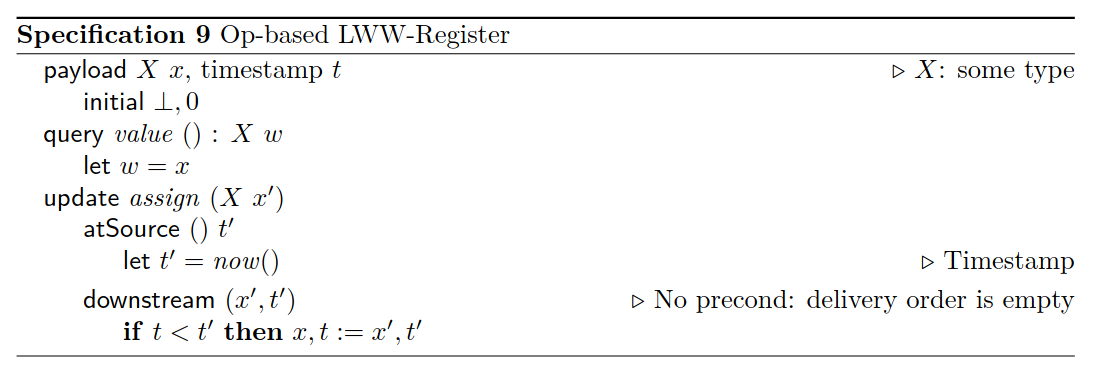
\includegraphics[width=\textwidth]{lww-definition}
    \caption{Last Writer Wins Register}
    \label{fig:lww-def}
\end{figure}

\TODO{Describe how we implemented it, and why we need to have a set of seen Timestamps to enforce uniqueness.}

\subsection{Grow-only Set and Two-Phase Set}

We have encoded the Grow-only Set (GSet) and Two-Phase Set (2PSet)
from \cite{baquero2017pure}. GSets only support adding items, and they
can be useful when logging events where logging is unimportant
(e.g. when storing IPs of clients visiting a web-site). 2PSets extend
GSets by supporting removals, but items that have been removed can
never be added again. Their definitions are shown in
\Cref{fig:get-def,fig:2pset-def}. The state of a GSet is just an
originally empty set of values of type $V$. It's only update function
is \texttt{add} which does nothing in the \texttt{prepare} stage, and
then updates the state by inserting the input element $v$ in the set
$s$. The two supported queries are asking for the elements and the
size of the state.

\begin{figure}[h]
    \centering
    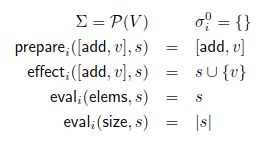
\includegraphics[width=0.5\textwidth]{grow-only-set-definition}
    \caption{Grow-only Set}
    \label{fig:gset-def}
\end{figure}

\begin{figure}[h]
    \centering
    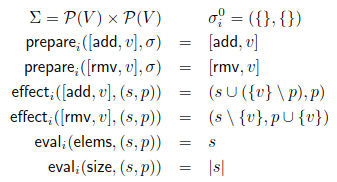
\includegraphics[width=0.5\textwidth]{2pset-definition}
    \caption{Two-Phase Set}
    \label{fig:2pset-def}
\end{figure}

\subsection{Graph CRDTs}

Say some things about the graph in section 5 of
\cite{shapiro2011conflict} and specification 16 from
\cite{shapiro2011comprehensive}.

\TODO{Describe where we got stuck and why.}

%% Bibliography
\bibliography{./draft}
\bibliographystyle{plain}



\end{document}
